\subsection{Соединения кислорода и родственные им соединения серы, способы получения, химическое поведение, электронное и геометрическое строение молекул.}

\subsubsection*{Кислород}

\textbf{Способы получения}
 
 Лабораторные:
 
$$H_2O_2 \rightarrow H_2O + O_2 (MnO_2)$$
$$KMnO_4 \rightarrow K_2MnO_4 + MnO_2 + O_2$$
$$KClO_3 \rightarrow KCl + O_2$$
$$KNO_3 \rightarrow KNO_2 + O_2$$

Промышленные:

Из воздуха на мембранах

$$H_2O \rightarrow H_2 + O_2$$

\textbf{Химические свойства}

1) Окисляет металлы и неметаллы (кроме легких галогенов, инертных газов и Au, Pt)

$$P_4 + O_2 \rightarrow P_2O_5$$
$$Na + O_2 \rightarrow Na_2O_2$$

2) Окисляет органические и неорганические соединения

$$E_1E_2 + O_2 \rightarrow E_{1x}O_y + E_{2z}O_{\alpha}$$
$$NeMeH + O_2 \rightarrow NeMe_xO_y + H_2O$$
$$C_xH_y + O_2 \rightarrow CO_2 + H_2O$$

3) Окисляется сильными окислителями

$$O_2 + PtF_6 \rightarrow [O_2]^+[PtF_6]$$

\textbf{Электронное и геометрическое строение}

Линейная молекула

Может быть триплетном (а) и возбужденном (б) состоянии

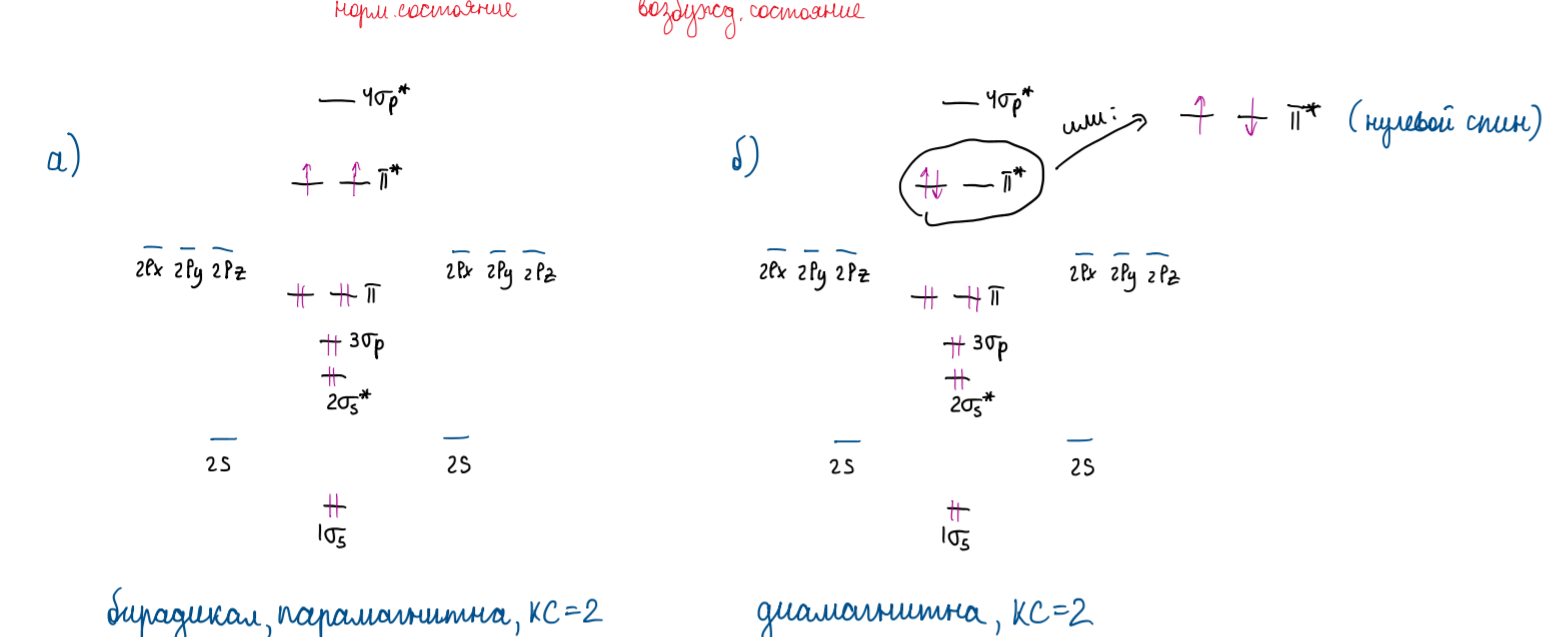
\includegraphics[scale=0.65]{images/6v1.png}

\subsubsection*{Озон}

\textbf{Способы получения}

1) Озонирование воздуха

2) При действии тихого электрического разряда на $O_2$

$$3O_2 \rightarrow 2O_3$$

\textbf{Химические свойства}

Сильнейший окислитель (сильнее $O_2$)

$$O_3 + 2H^+ + 2e^- \rightarrow O_2 + H_2O$$
$$O_3 + H_2O + 2e \rightarrow O_2 + 2OH^-$$
$$O_3 + S + H_2O \rightarrow KOH + O_2 + I_2$$
$$O_3 + KOH \rightarrow KO_3 + O_2 + I_2$$

\textbf{Электронное и геометрическое строение}

Изогнута(угол О-О-О)= $116,8^{\circ}$

$d(O=O)_{O_2}< d(O\simeq O)_{O_3}<d(O-O)_{H_2O_2}$

Каждый атом О образует одну связь с соседним атомом р-электрона. Отслаьные р-орбитали комбнируются с образованием одной несвязывающей и одной разрыхляющей орбиталей. Количество электронов точно соответствует заселению связывающей и несвязывающей МО.

Молекула диамагнитна

\subsubsection*{Сера}

Аллотропия S:

- ромбическая $S_8$ устойчивая\\
- Моноклинная $S_8$\\
- Пластическая $S_n$

\textbf{Способы получения}

Неполное сгорание $MeS$ и $H_2S$

$$MeS + O_2 \rightarrow MeO + S$$
$$H_2S + O_2 \rightarrow S + H_2O$$
$$H_2S + SO_2 \rightarrow S+ H_2O$$

\textbf{Химические свойства}

1) С простыми веществами
$$S + O_2 \rightarrow SO_2$$
$$P + S \rightarrow P_2S_3$$
$$S+F_2 \rightarrow SF_6$$
$$Me + S \rightarrow MeS$$

2) Окисление

$$S + HClO_3 + H_2O \rightarrow H_2SO_4 + HCl$$

3) Образование поликатионов

$$S_8 + AsF_5 \rightarrow [S_8]^{2+}[AsF_6]_2^- + AsF_3(SO_2 liq)$$

4) Диспропорционирование

$$S + Na_2SO_3 \rightarrow Na_2S_2O_3$$
$$S + MeOH \rightarrow MeS + MeSO_3 + H_2O$$

\textbf{Электронное и геометрическое строение}

Устойчивые гомоцепи -S-S- (зигзагообразно)\\
$S_8$ - циклическая молекула, форма короны\\
Ромбическая - форма прямоугольного параллелепипеда;\\
моноклинная - скошенный параллелепипед;\\
пластическая - скрученные спиральные цепи.

\subsubsection*{Вода}

\textbf{Способы получения}


1) Продукт в огромном количестве реакции

2) Физические методы (дистилляция)

3) $H_2 + O_2 \rightarrow H_2O$

\textbf{Химические свойства}

1) Автопротолиз

$$2H_2O \leftrightarrows H_3O^+ + OH^-$$

2) Окислитель

$$H_2O + Al_{amalgama}\rightarrow Al(OH)3 + H_2$$

3) Восстановитель

$$H_2O + CoF_3 \rightarrow CoF_2 + O_2 + HF$$

\textbf{Электронное и геометрическое строение}

Угловая форма ($AB_2E_2$  по Гиллеспи)

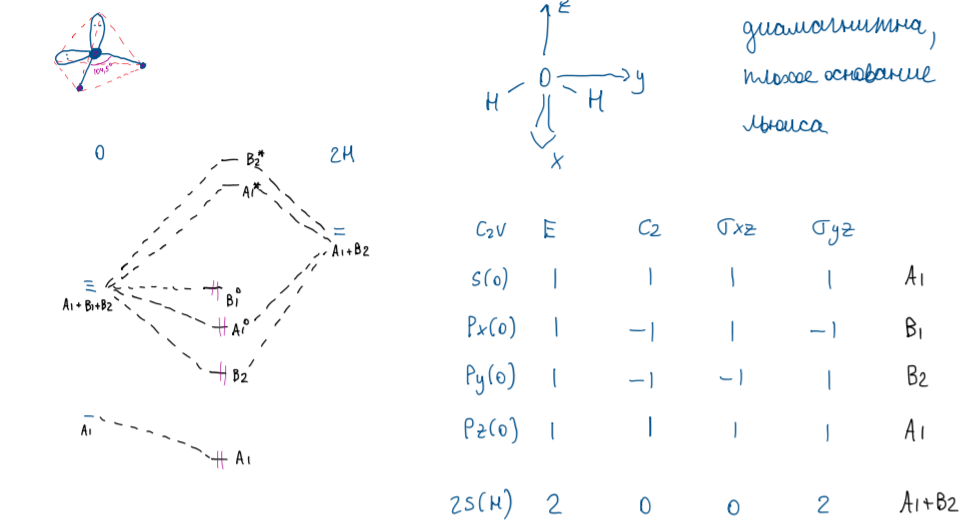
\includegraphics{images/6v2.png}

\subsubsection*{Пероксид водорода}

\textbf{Методы получения}

$$BaO_2 + H_2SO_4 \rightarrow BaSO_4\downarrow + H_2O_2$$
$$ (CH_3)_2CHOH + O_2 \rightarrow (CH_3)_2CO + H_2O_2$$

Окисление гидроантрахинонаксилородом воздуха в органическом растворителе

\textbf{Химические свойства}

1) Разложение
$$H_2O_2 \rightarrow H_2O + O_2$$

2) Слабая кислота

$$H_2O_2 + H_2O \rightarrow H_3O^+ + HO_2^-$$
$$H_2O_2 + NaOH \rightarrow Na_2O_2 + H_2O$$

3) $Red/ox$ свойства

- сильный окислитель в кислой среде

$$NaI + H_2O_2 + H_2SO_4 \rightarrow I_2 + Na_2SO_4 + H_2O$$

- Восстановитель в кислой среде

$$KMnO_4 + H_2O_2 + H_2SO_4 \rightarrow MnSO_4 + K_2SO_4 + H_2O + O_2$$

- Окислитель в щелочной среде

$$Cr(OH)_3 + H_2O_2 + KOH \rightarrow K2CrO_4 + H_2O$$

- Восстановитель в щелочной среде

$$KOH + Cl_2 + H_2O_2 \rightarrow KCl + O_2 + H_2O$$

- Гетерогенный окислитель

$$PbS_{tv.} + H_2O_2 \rightarrow PbSO_4{tv.} + H_2O$$

\textbf{Электронное и геометрическое строение}

Строение обусловлено взаимным отталкиванием между неподеленными парами $e^-$ O и $e^-$ связи $O-H$

Молекула сильно полярна

НЭП 0 $\Rightarrow$ Д/А связи

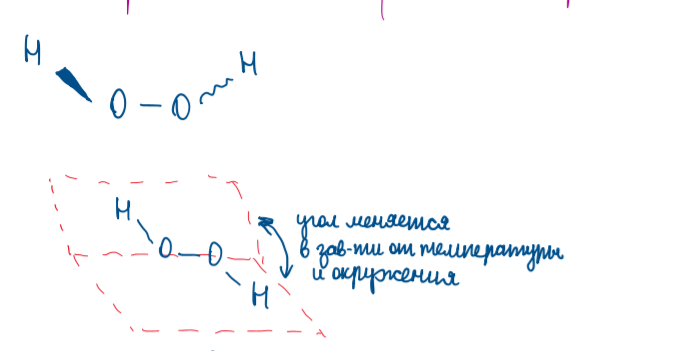
\includegraphics[scale=0.95]{images/6v3.png}

\subsubsection*{Сероводород}

Пиросульфаны $H_2S_n$ термодинамически неуйстойчивы, например,  $H_2S_2$ разлагается водой на $S$ и $H_2S$; проявляет окислительные свойства, строение близко к $H_2O_2$

\textbf{Способы получения}

$$FeS + HCl \rightarrow FeCl_2 + H_2S$$

Гидролиз $CaS, BaS, Al_2S_3$

$$H_2 + S \rightarrow H_2S (600^{\circ})$$

\textbf{Химические свойства}

1) Слабая кислота в растворе

$$H_2S + CuSO_4 \rightarrow CuS\downarrow + H_2SO_4$$
$$NaOH + H_2S \rightarrow NaHS (Na_2S) + H_2O$$

2) Окисление

$$H_2S + I_2 \rightarrow HI + S$$
$$H_2S + SO_2 \rightarrow S+ H_2O$$
$$H_2S + H_2SO_4 + KMnO_4 \rightarrow K_2SO_4 + H_2O + S$$
$$H_2S + O_2 \rightarrow SO_2 + H_2O$$

\textbf{Электронное и геометрическое строение}

Угловая молекула, полярна\\
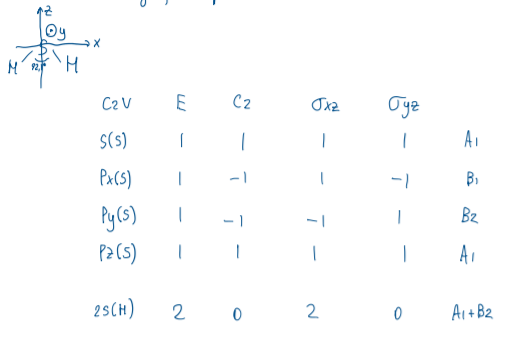
\includegraphics{images/6v4.png}
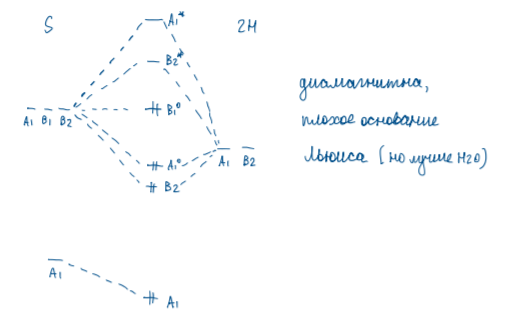
\includegraphics{images/6v5.png}

\subsubsection*{Оксиды - большое многообразие (кислотные, основные, амфотерные)}

\textbf{Способы получения}\\
1) Взаимодействие простых веществ

2) Термическое разложение некоторых солей, кислот, оснований

$$CaCO_3 \rightarrow CaO + CO_3$$
$$Cu(OH)_2 \rightarrow CuO + H_2O$$
$$H_2CO_3 \leftrightarrows H_2O _ CO_2$$

3) Горение бинарных соединений

\textbf{Химические свойства}

1) Если элемент не в высшей степени окисления, то окисление

$$SO_3 + O_2 \rightarrow SO_3$$

2) Основные оксиды:

- с $H_2O$ (Щ и Щ/М металлы кроме Mg, Be)

- C $H^+$

- С кислотными и амфотерными оксидами

3) Амфотерные оксиды:

- С $H^+$ и $OH^-$

- С основными и кислотными оксидами

\textbf{Электронное и геометрическое строение}

Многообразие форм.

К примеру, оксиды p и d элементов в низких с.о. - полимерные структуры;\\
в высоких с.о - молекулярные структуры, часто повышенная кратность связи\\
Некоторые оксиды задают структурные типы:\\
Рутил $TiO_2$

КЧ($Ti^{4+}$)=6; КЧ = ($O^{2-}$)=3

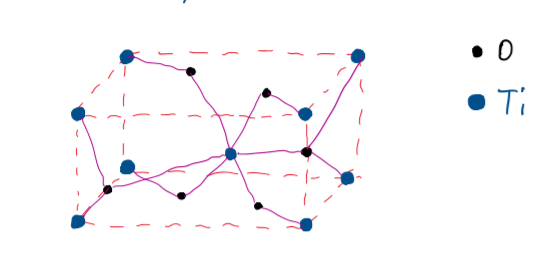
\includegraphics{images/6v6.png}

\subsubsection*{Сульфиды}

\textbf{Способы получения}

1) Ме + S

$$Fe + S \rightarrow FeS$$
$$CdO + S \rightarrow CdS + SO_2$$
$$Ga + H_2S \rightarrow Ga_2S_3 + H_2$$

2) Обменные реакции

$$ZnCl_2 + Na_2S \rightarrow ZnS + NaCl$$

\textbf{Химические свойства}

1) Горение

$$MeS + O_2 \rightarrow MeO + S$$
$$MeS + O_2 \rightarrow MeO + SO_2$$

2) Окисление

$$CuS + HNO_{3(konc)} \rightarrow CuSO_4 + NO_2 + H_2O$$

3) Растворимые сульфиды - с солями тяжелых металлов

4) С сильными кислотами до $H_2S\uparrow$ (некоторые растворимы в кислотах : $PbS, CuS, Ag_2S, HgS, CoS, Li_2S$)

5) Необратимый гидролиз до основания и $H_2S$

\textbf{Электронное и геометрическое строение}

$M_2S$ - структура типа флюорита (каждый атом S окружен кубом из 8 атомов Me, а каждый атом Me - тетраэдром из 4 атомов S)

$MS$ -структура типа $NaCl$ (каждый атом Ме и S окружен октаэдром из атомов другого сорта)
